\documentclass[12pt]{article}
 
\usepackage[margin=1in]{geometry} 
\usepackage{amsmath,amsthm,amssymb}

\usepackage[brazilian]{babel}
\usepackage[utf8]{inputenc}
\usepackage[T1]{fontenc}
\usepackage{graphicx}         %pacote para incluir figuras tipo eps
\usepackage{xcolor}
\usepackage{float} 
\usepackage{epstopdf}
\usepackage{longtable}
\usepackage{subcaption}

 
 %Matlab code in latex 
\usepackage[final]{listings}
\usepackage{color} %red, green, blue, yellow, cyan, magenta, black, white
\definecolor{mygreen}{RGB}{28,172,0}
\definecolor{mylilas}{RGB}{170,55,241}
\lstdefinestyle{myMatlab}
{
language=matlab,frame=single, basicstyle=\small\ttfamily,breaklines=true,%
morekeywords={matlab2tikz}, keywordstyle=\color{blue}, morekeywords=[2]{1}, keywordstyle=[2]{\color{black}}, commentstyle=\color{mygreen}, stringstyle=\color{mylilas}, identifierstyle=\color{black}, showstringspaces=false,%without this there will be a symbol in the places where there is a space
numbers=left, numberstyle={\scriptsize \color{black}},% size of the numbers
numbersep=9pt, % this defines how far the numbers are from the text
% emph=[1]{for,end,break},emphstyle=[1]\color{red}, %some words to emphasise
% emph=[2]{word1,word2}, emphstyle=[2]{style},
}
 
\newcommand{\N}{\mathbb{N}}
\newcommand{\Z}{\mathbb{Z}}
 
\newenvironment{theorem}[2][Theorem]{\begin{trivlist}
\item[\hskip \labelsep {\bfseries #1}\hskip \labelsep {\bfseries #2.}]}{\end{trivlist}}
\newenvironment{lemma}[2][Lemma]{\begin{trivlist}
\item[\hskip \labelsep {\bfseries #1}\hskip \labelsep {\bfseries #2.}]}{\end{trivlist}}
\newenvironment{exercise}[2][Exercício]{\begin{trivlist}
\item[\hskip \labelsep {\bfseries #1}\hskip \labelsep {\bfseries #2.}]}{\end{trivlist}}
\newenvironment{reflection}[2][Reflection]{\begin{trivlist}
\item[\hskip \labelsep {\bfseries #1}\hskip \labelsep {\bfseries #2.}]}{\end{trivlist}}
\newenvironment{proposition}[2][Proposition]{\begin{trivlist}
\item[\hskip \labelsep {\bfseries #1}\hskip \labelsep {\bfseries #2.}]}{\end{trivlist}}
\newenvironment{corollary}[2][Corollary]{\begin{trivlist}
\item[\hskip \labelsep {\bfseries #1}\hskip \labelsep {\bfseries #2.}]}{\end{trivlist}}
 
\begin{document}
 
% --------------------------------------------------------------
%                         Start here
% --------------------------------------------------------------
 
\title{Exercício 03}
\author{Renan Salles de Freitas\\
CPE 723 - Otimização Natural}
 
\maketitle
 
\begin{exercise}{1.a}
O código MatLab para gerar o gráfico está abaixo:
\lstinputlisting[style=myMatlab]{matlab/ex1_a.m}

\begin{figure}[H]
    \centering
    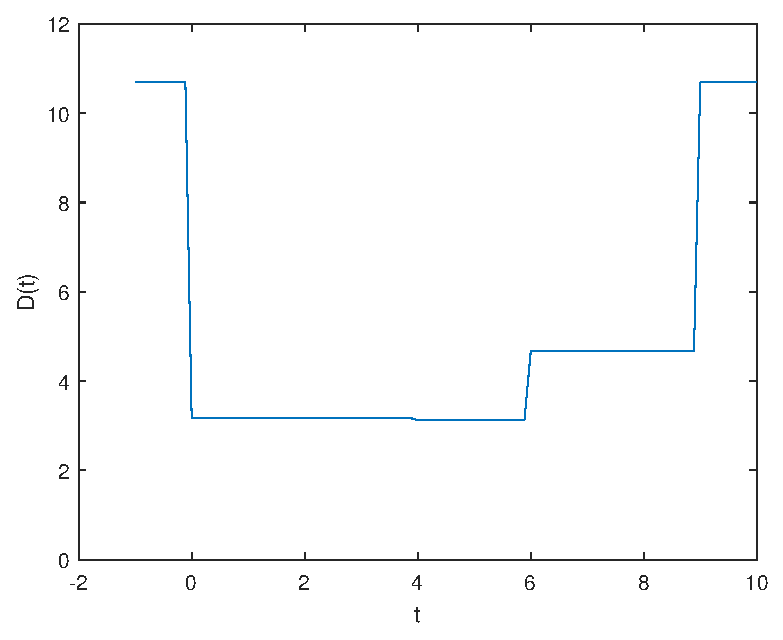
\includegraphics[width=0.5\textwidth]{figs/ex1a.eps}
\end{figure}
\end{exercise}

\begin{exercise}{1.b}
No algoritmo \textit{Deterministic Annealing}, temos que a condição de partição
é dada pela fórmula:

\begin{align*}
p_{y|x} &= \frac{e^{-d_{xy}/T}}{\mu_x}
\end{align*}

Onde $d_{xy}$ é a distância quadrática entre o centróide $y$ e o dado $x$:

\begin{align*}
d_{xy} &= \begin{bmatrix}
(x_1-y_1)^2 & (x_2-y_1)^2 & (x_3-y_1)^2 & (x_4-y_1)^2 \\
(x_1-y_2)^2 & (x_2-y_2)^2 & (x_3-y_2)^2 & (x_4-y_2)^2
\end{bmatrix} = \begin{bmatrix} 9 & 1 & 9 & 36 \\
11.56 & 0.36 & 6.76 & 31.36 \end{bmatrix}
\end{align*}

E $\mu_x = \sum_y e^{-d_{xy}/T}$.

Dessa forma, podemos calcular a matriz de probabilidade conjunta:
\begin{align*}
p_{y|x} = \begin{bmatrix}
0.9282 & 0.3452 & 0.0962 & 0.0096\\
0.0718 & 0.6548 & 0.9038 & 0.9904
\end{bmatrix}
\end{align*}

\lstinputlisting[style=myMatlab]{matlab/ex1_b.m}

\end{exercise}

\begin{exercise}{1.c}
Podemos calcular $D$ a partir do somatório:
\begin{align*}
D &= \sum_x p(x) \sum_y p(y|x)d(x,y) \\
&= \frac{1}{4} (p_{1|1} d(1,1) + p_{2|1}
d(1,2) + p_{2|1} d(2,1) + p_{2|2} d(2,2) + \\
&+ p_{3|1} d(3,1) + p_{3|2} d(3,2) +
p_{4|1} d(4,1) + p_{4|2} d(4,2)) \\
&= 12.0361
\end{align*}

\lstinputlisting[style=myMatlab]{matlab/ex1_c.m}
\end{exercise}

\begin{exercise}{1.d}
A condição de centróide é regida pela fórmula:
\begin{align*}
y_k &= \frac{\sum_x p_{k|x} x}{\sum_x p_{k|x}}
\end{align*}

Logo:
\begin{align*}
y_1 &= \frac{\sum_x p_{1|x} x}{\sum_x p_{1|x}} \\
&= \frac{p_{1|1} x_1 + p_{1|2} x_2 + p_{1|3} x_3 + p_{1|4} x_4}{p_{1|1} +
p_{1|2} + p_{1|3} + p_{1|4}} \\
&= 1.4822
\end{align*}

\begin{align*}
y_2 &= \frac{\sum_x p_{2|x} x}{\sum_x p_{2|x}} \\
&= \frac{p_{2|1} x_1 + p_{2|2} x_2 + p_{2|3} x_3 + p_{2|4} x_4}{p_{2|1} +
p_{2|2} + p_{2|3} + p_{2|4}} \\
&= 6.4698
\end{align*}

\lstinputlisting[style=myMatlab]{matlab/ex1_d.m}
\end{exercise}

\begin{exercise}{1.e}
Para este exercício, usamos o código de Matlab abaixo:
\lstinputlisting[style=myMatlab]{matlab/ex1_e.m}

E obtemos:
\begin{align*}
p_{y|x} = \begin{bmatrix}
1 & 0.0017 & 0 & 0\\
0 & 0.9983 & 1 & 1
\end{bmatrix}
\end{align*}

\begin{align*}
D &= 11.8703
\end{align*}

\begin{align*}
Y &= \begin{bmatrix}
0.0066 \\ 6.3346
\end{bmatrix}
\end{align*}
\end{exercise}

\begin{exercise}{1.f}
Para este exercício, usamos o código de Matlab abaixo:
\lstinputlisting[style=myMatlab]{matlab/ex1_f.m}

E obtemos:
\begin{align*}
p_{y|x} = \begin{bmatrix}
0.5128 & 0.4968 & 0.4888 & 0.4768\\
0.4872 & 0.5032 & 0.5112 & 0.5232
\end{bmatrix}
\end{align*}

\begin{align*}
D &= 13.0881
\end{align*}

\begin{align*}
Y &= \begin{bmatrix}
4.6635 \\ 4.8344
\end{bmatrix}
\end{align*}
\end{exercise}

\begin{exercise}{1.g}
Para temperaturas baixas ($T=0.1$), o problema cai em uma situação de
\textit{hard-clustering}, isto é, a matriz de probabilidades conjuntas
da condição de partição ($p_{y|x}$) possui apenas valores 0 e 1, não havendo a
estocacidade do algoritmo e os centróides ficam em $y = [0
\quad 6.333]$, já que o algoritmo separa os dados mais próximos para os
clusters: $y_1 = 0$ e $y_2 = (4 + 6 + 9)/3 = 6.333$.

Para temperaturas altas, o problema está
próximo da máxima entropia, e os valores da matriz de probabilidades conjuntas
ficam em torno de $0.5$ para todo $y|x$. Isso pode ser percebido pelo decaimento
rápido das exponenciais. Neste caso, há a formação de apenas um cluster: $y_1 =
y_2 = \sum_x X / 4 = 4.75$.

Para o caso de temperaturas intermediárias $T = 1$,, podemos observar o
comportamento de \textit{soft-clustering} para o caso $p_{y|x_2}$, na matriz de
probabilidade conjunta. Porém a temperatura se assemelha mais ao caso quando
$T=0.1$.

\end{exercise}

\begin{exercise}{2}
Para este exercício vamos utilizar a função Rosenbrock para N = 20:
\begin{align*}
f(\textbf{x}) = \sum_{i=1}^{N-1} 100(x_{i+1}-x_i^2)^2 + (x_i-1)^2
\end{align*}
O mínimo está em $\text{x}_\text{min}= \textbf{1}$ e $\text{J}_\text{min} =
0$. 
O código MatLab para SA está abaixo:
\lstinputlisting[style=myMatlab]{matlab/ex2.m}

A função custo:
\lstinputlisting[style=myMatlab]{matlab/J.m}

Encontramos:
\begin{align*}
\text{x}_\text{min} &= \begin{bmatrix}
0.9757 \\ 0.9996 \\ 1.0407 \\ 1.0047 \\ 1.0362 \\ 1.0222 \\ 1.0272 \\ 1.0079 \\   
1.0393 \\ 1.0419 \\ 1.0175 \\ 0.9761 \\ 0.9383 \\ 0.9927 \\ 0.9859 \\ 0.9470 \\   
0.9995 \\ 0.9951 \\ 0.9385 \\ 0.9177
\end{bmatrix}
\end{align*}
e $\text{J}_\text{min} = 5.4474$.

\begin{figure}[H]
    \centering
    \begin{subfigure}[b]{0.45\textwidth}
        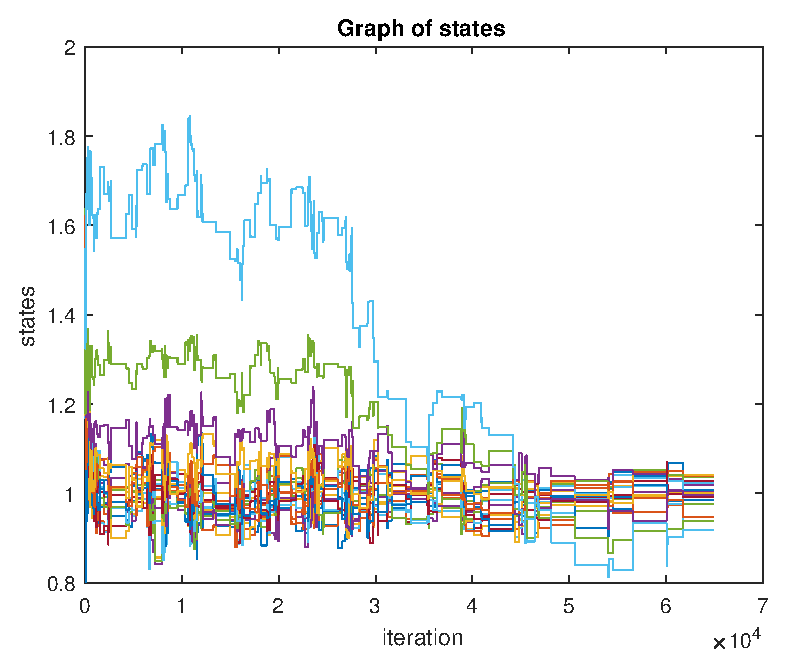
\includegraphics[width=\textwidth]{figs/ex3_states.eps}
    \end{subfigure}
    ~ 
    \begin{subfigure}[b]{0.45\textwidth}
        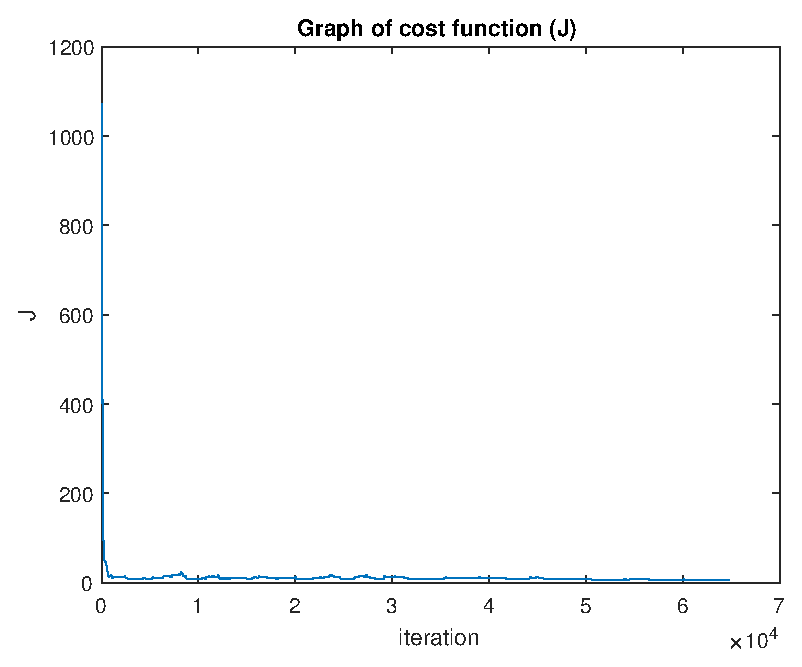
\includegraphics[width=\textwidth]{figs/ex3_j.eps}
    \end{subfigure}
\end{figure}

Verificou-se que o SA teve certa dificuldade em encontrar o mínimo global pelo
grande número de mínimos locais. O algoritmo desenvolvido possui mais iterações
nas temperaturas altas e menos nas temperaturas baixas. Dessa forma, o
algoritmo realiza $30.000$ iterações para $T_0=1$ e reduz oo número de
iterações logaritmicamente, como a temperatura. Além disso, o algoritmo é
sensível à perturbação, resfriamento, e condição inicial.
\end{exercise}
 
\end{document}
              
